\chapter{Results}\label{ch:results}

This chapter presents the delivered results and user interface achievements of the LiveSpot application. The results demonstrate successful delivery of a functional cross-platform social networking application with comprehensive UI/UX delivery, feature integration, and performance optimization across mobile and web platforms.

\section{User Interface Results}\label{sec:ui_results}

This section showcases the delivered user interface results, demonstrat
ful achievement of intuitive, responsive, and accessible design across all supported platforms. The UI results highlight the success of cross-platform consistency, user experience optimization, and comprehensive feature integration.

\subsection{UI/UX Design}\label{subsec:ui_ux_design}

The LiveSpot application delivers comprehensive UI/UX design that prioritizes user accessibility, cross-platform consistency, and intuitive navigation. The delivered interface provides cohesive user experience across Android, iOS, and web platforms with consistent design language.

\subsection{Cross-Platform Design Achievement}\label{subsec:cross_platform_design}

The application successfully delivers visual and functional consistency across Android, iOS, and web platforms. The achieved design system demonstrates consistent theming, responsive layouts, and platform-appropriate adaptations while maintaining brand identity.

\textbf{Theming Results:}
The delivered theming system provides seamless light and dark mode support across all platforms. Users receive elegant dark themes on mobile platforms and clean, accessible light themes on web platforms, both maintaining consistent branding and accessibility compliance.

\subsection{Authentication Interface Results}\label{subsec:auth_interface_results}

The authentication system delivers comprehensive user onboarding with complete registration, login, and password recovery interfaces. The delivered solution provides smooth user experience with clear visual feedback and intuitive form interactions.

\paragraph{Account Creation Flow Results}
The delivered account registration provides complete user onboarding from welcome screen through account creation and email verification. The mobile interface showcases the achieved dark theme with clear visual hierarchy and user guidance.

\textbf{Mobile Interface (Android):}
\begin{figure}[!htbp]
    \centering
    \subfigure[Welcome Screen]{
        \includegraphics[width=0.32\textwidth]{figures/ui/get_started_android.jpeg}
    }%
    \subfigure[Create Account]{
        \includegraphics[width=0.32\textwidth]{figures/ui/create_account_android.jpeg}
    }%
    \subfigure[Email Verification]{
        \includegraphics[width=0.32\textwidth]{figures/ui/verify_email_signup_android.jpeg}
    }
    \caption{Account Creation Flow on Android---Dark Theme Achievement}\label{fig:android_account_creation}
\end{figure}

The delivered account creation system successfully provides:

\textbf{Completed Registration Features:}
\begin{itemize}
    \item \textbf{Multiple Authentication Options:} Successfully delivered traditional email/password and Google OAuth integration with seamless user experience
    \item \textbf{Form Validation:} Delivered real-time password strength indicators and comprehensive input validation with immediate user feedback
    \item \textbf{Email Verification:} Implemented automated verification system with format validation and confirmation email delivery
    \item \textbf{Cross-Platform Consistency:} Achieved consistent registration experience across mobile and web platforms
    \item \textbf{User Experience Optimization:} Delivered intuitive form layouts with clear progress indicators and error messaging
\end{itemize}

\textbf{Web Platform Results:}
The completed web interface demonstrates responsive design adaptation for desktop and tablet screens with optimized layouts and accessibility features.

\begin{figure}[!htbp]
    \centering
    \includegraphics[width=0.8\textwidth]{figures/ui/create_account_web.png}
    \caption{Account Creation on Web---Light Theme Responsive Design}\label{fig:web_account_creation}
\end{figure}

\paragraph{Login Interface Results}
The completed login interface delivers secure user authentication with consistent branding and optimized form interactions across mobile and web platforms.

\textbf{Web Interface:}
\begin{figure}[!htbp]
    \centering
    \includegraphics[width=0.7\textwidth]{figures/ui/login_web.png}
    \caption{Login Interface on Web---Light Theme Design}\label{fig:web_login}
\end{figure}

\textbf{Mobile Interface (Android):}
\begin{figure}[!htbp]
    \centering
    \includegraphics[width=0.27\textwidth]{figures/ui/login_android.jpeg}
    \caption{Login Interface on Android---Dark Theme Achievement}\label{fig:android_login}
\end{figure}

\paragraph{Password Recovery Results}
The delivered password recovery system provides secure multi-step account recovery with clear visual feedback and user guidance throughout the process.

\textbf{Mobile Interface (Android):}
\begin{figure}[!htbp]
    \centering
    \subfigure[Reset Request]{
        \includegraphics[width=0.27\textwidth]{figures/ui/forget_password.jpeg}
    }
    \hspace{0.02\textwidth}
    \subfigure[Verification Code]{
        \includegraphics[width=0.27\textwidth]{figures/ui/forget_password_verify_android.jpeg}
    }
    \caption{Password Recovery Flow on Android---Reset Process}\label{fig:android_password_recovery}
\end{figure}

\subsection{Application Interface Results}\label{subsec:app_interface_results}

The core application interfaces demonstrate successful integration of complex functionality with clean visual design and optimized user interaction patterns. The delivered solution provides sophisticated features through intuitive interface design.

\paragraph{Home Feed Interface Results}
The delivered home interface successfully provides a location-aware news feed with integrated map functionality, story features, and intelligent content filtering. The achievement demonstrates seamless integration of complex features through clean, intuitive design.

\textbf{Mobile Interface (Android):}
\begin{figure}[!htbp]
    \centering
    \subfigure[Main Feed]{
        \includegraphics[width=0.45\textwidth]{figures/ui/home_android_1.jpeg}
    }
    \hspace{0.05\textwidth}
    \subfigure[Alternative View]{
        \includegraphics[width=0.45\textwidth]{figures/ui/home_2android.jpeg}
    }
    \caption{Home Feed Interface on Android---Dark Theme Achievement}\label{fig:android_home}
\end{figure}

\clearpage
\textbf{Web Platform Achievement:}
The delivered web platform provides optimized experience for larger screens with enhanced navigation and responsive content discovery features.

\begin{figure}[!htbp]
    \centering
    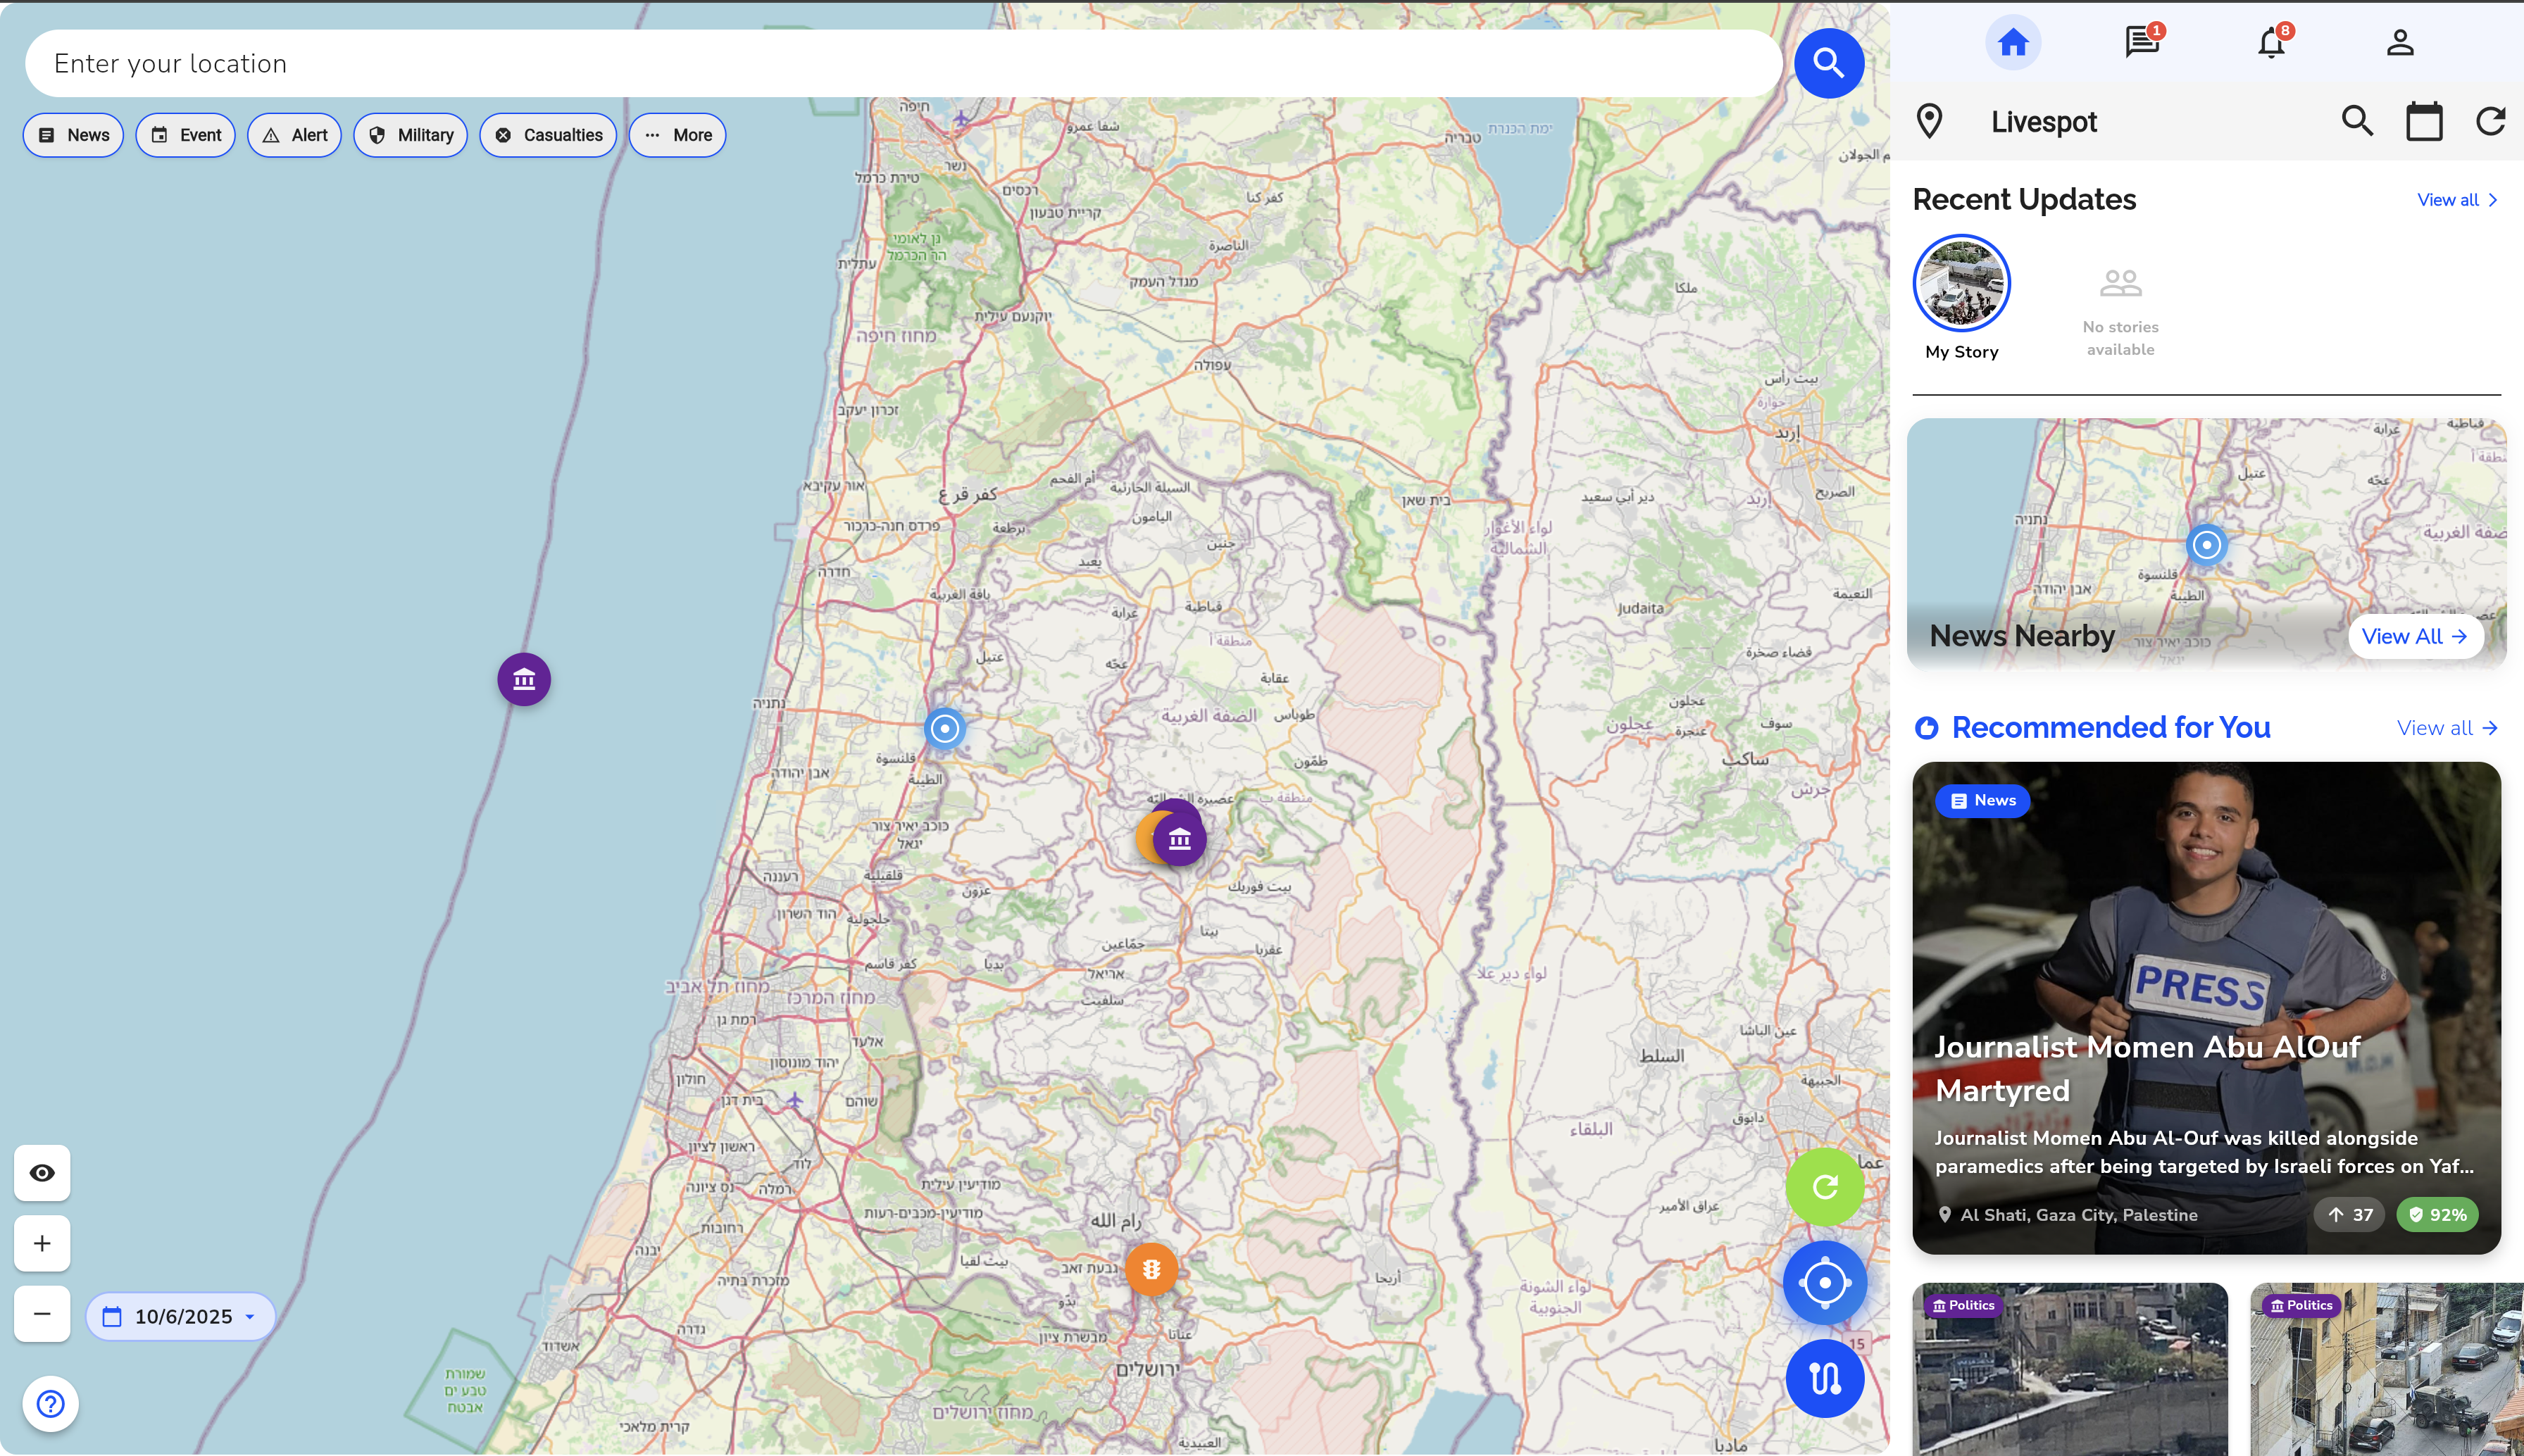
\includegraphics[width=1\textwidth]{figures/ui/home_wb.png}
    \caption{Home Feed Interface on Web---Light Theme Responsive Design}\label{fig:web_home}
\end{figure}

\paragraph{Profile Management Results}
The delivered profile management system provides comprehensive user account features with optimized readability and interaction design across mobile and web platforms.

\textbf{Mobile Achievement:}
The delivered mobile profile system provides comprehensive account customization, settings configuration, and privacy controls through intuitive interface design.

\begin{figure}[!htbp]
    \centering
    \subfigure[Settings Overview]{
        \includegraphics[width=0.32\textwidth]{figures/ui/Settings_android.jpeg}
    }%
    \subfigure[Profile View]{
        \includegraphics[width=0.32\textwidth]{figures/ui/profile_page_android.jpeg}
    }%
    \subfigure[Edit Profile]{
        \includegraphics[width=0.32\textwidth]{figures/ui/edit_profile_android.jpeg}
    }
    \caption{Profile Management on Android---Comprehensive User Account Features}\label{fig:android_profile_management}
\end{figure}

\begin{figure}[!htbp]
    \centering
    \subfigure[Change Password]{
        \includegraphics[width=0.32\textwidth]{figures/ui/change_password_settings_android.jpeg}
    }
    \hspace{0.05\textwidth}
    \subfigure[Notification Settings]{
        \includegraphics[width=0.32\textwidth]{figures/ui/notfications settings_android.jpeg}
    }
    \caption{Profile Security and Notification Management on Android}\label{fig:android_profile_security}
\end{figure}

The mobile profile interface demonstrates achieved functionality:
\begin{itemize}
    \item \textbf{Settings Panel Achievement:} Delivered complete account management with organized sections for appearance, account information, notifications, privacy, and data controls
    \item \textbf{Theme Customization Achievement:} Fully functional light mode, dark mode, and system default options with visual indicators
    \item \textbf{Security Features Achievement:} Working verification requests, email/password management, and security controls
    \item \textbf{Advanced Notification Achievement:} Successfully delivered granular control over friend requests, events, reminders, nearby events, system notifications, follow notifications, and location-based verification alerts
    \item \textbf{Privacy Controls Achievement:} Functional profile visibility settings, location sharing preferences, and notification management
    \item \textbf{Profile Editing Achievement:} Completed full name, bio, location, and profile picture customization with intuitive form design
    \item \textbf{Data Management Achievement:} Working cache clearing, data download requests, and account deactivation/deletion functionality
\end{itemize}

\textbf{Delivered Notification Features:}
The delivered notification settings demonstrate LiveSpot's comprehensive approach to user communication:
\begin{itemize}
    \item \textbf{Social Notifications Implementation:} Successfully delivered friend requests, follow/unfollow activities, and social engagement alerts
    \item \textbf{Event Management Achievement:} Completed event invitations, reminders, confirmations, and location-based event discovery functionality
    \item \textbf{Location Intelligence Implementation:} Working nearby events detection and "Still Happening" verification prompts for real-time event status updates
    \item \textbf{System Communication Achievement:} Functional app updates, important announcements, and platform notifications
    \item \textbf{Granular Control Implementation:} Successfully delivered individual toggle switches for each notification category with complete user customization capabilities
\end{itemize}
\clearpage

\textbf{Web Interface:}
\begin{figure}[!htbp]
    \centering
    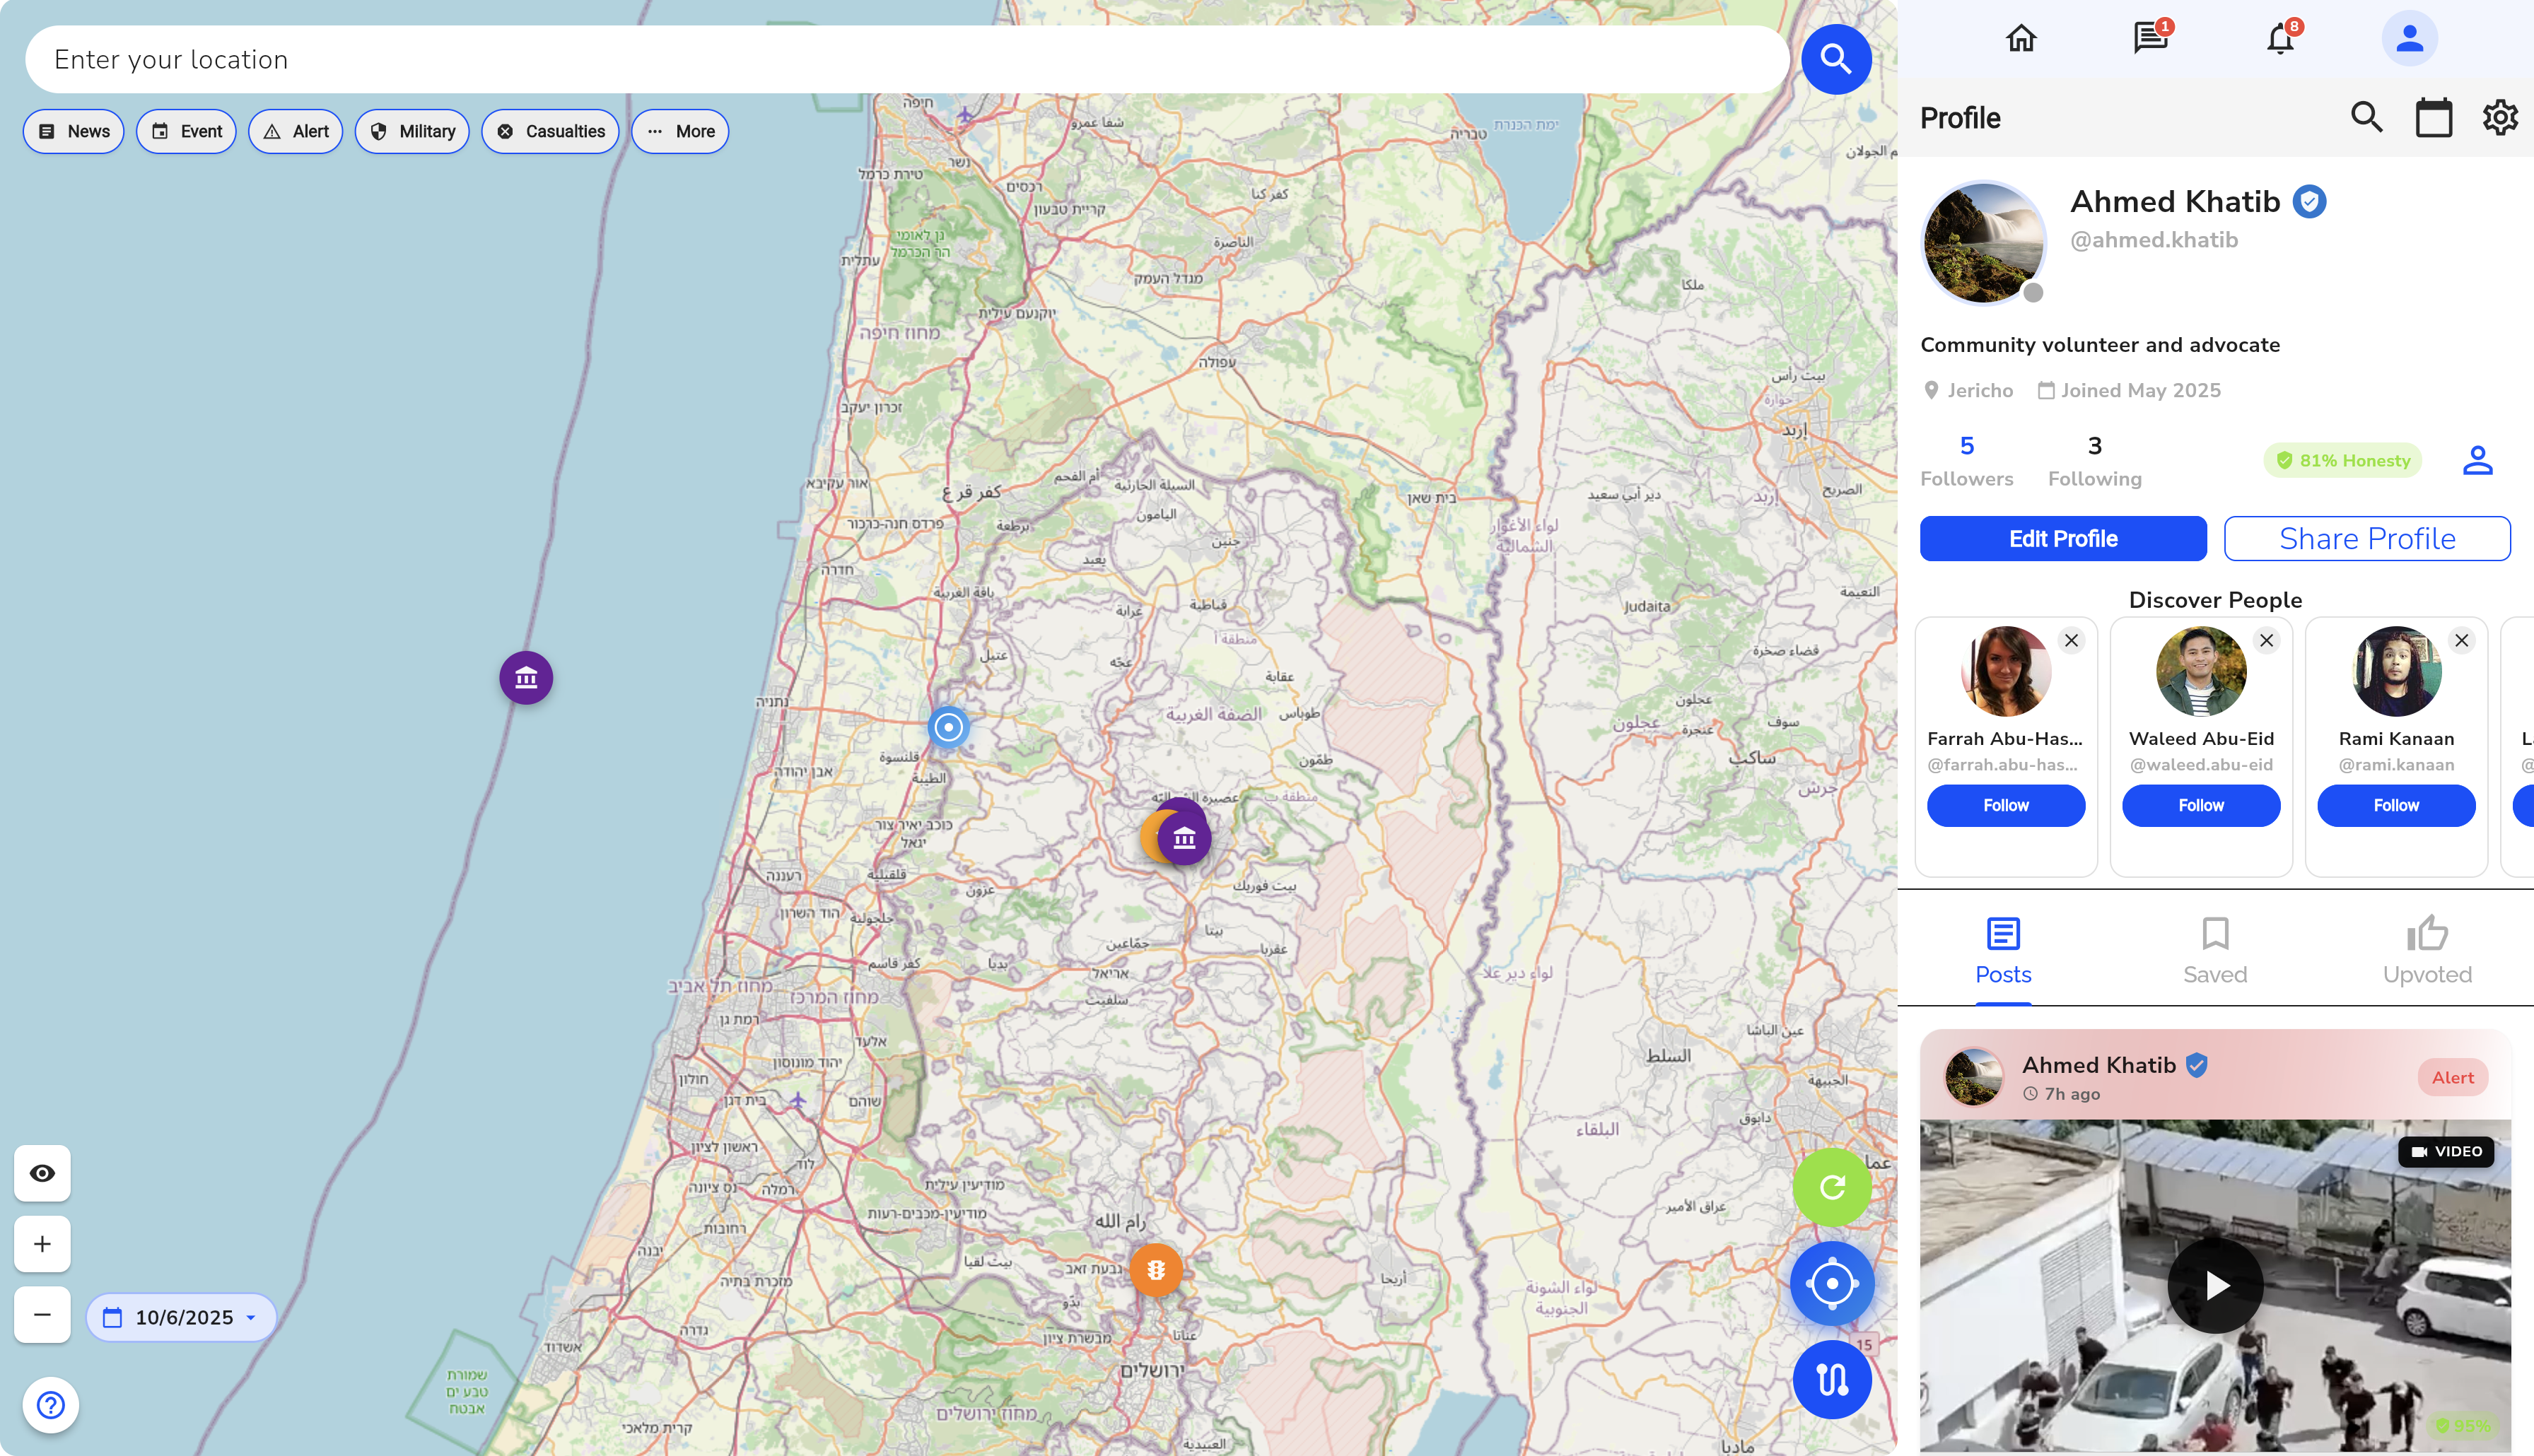
\includegraphics[width=0.9\textwidth]{figures/ui/profile_web.png}
    \caption{Profile Management on Web---Comprehensive User Interface}\label{fig:web_profile}
\end{figure}

\paragraph{Content Creation Results}
The delivered content creation system provides comprehensive post publishing with intelligent location detection, media attachment capabilities, and flexible scheduling. The interface successfully guides users through content creation while maintaining location-based context and community engagement focus.

\textbf{Mobile Interface (Android):}
\begin{figure}[!htbp]
    \centering
    \subfigure[Post Creation - Step 1]{
        \includegraphics[width=0.3\textwidth]{figures/ui/create post1_android.jpeg}
    }%
    \subfigure[Post Creation - Step 2]{
        \includegraphics[width=0.3\textwidth]{figures/ui/Long_create_Post2_android.jpeg}
    }%
    \subfigure[Date Selection]{
        \includegraphics[width=0.3\textwidth]{figures/ui/date_picker_homepage_android.jpeg}
    }
    \caption{Content Creation Flow on Android---Multi-Step Post Publishing}\label{fig:android_content_creation}
\end{figure}

The content creation system showcases several innovative features:
\begin{itemize}
    \item \textbf{Intelligent Location Detection:} Automatic location detection with manual override options for precise positioning
    \item \textbf{Media Integration:} Support for photos, videos, and quick attachment options with camera integration
    \item \textbf{Flexible Scheduling:} Comprehensive date and time selection for both immediate and scheduled publishing
    \item \textbf{Category Classification:} Intelligent content categorization with user confirmation and manual adjustment options
    \item \textbf{Privacy Controls:} Public/private posting options with clear visibility indicators
\end{itemize}
\clearpage
\paragraph{Camera Integration Results}
The application delivers seamless camera integration for immediate content capture and sharing, maintaining focus on real-time location-based reporting. The delivered unified camera interface supports both photo and video capture with intelligent mode switching and intuitive controls.

\textbf{Mobile Interface (Android):}
\begin{figure}[!htbp]
    \centering
    \subfigure[Photo Mode]{
        \includegraphics[width=0.3\textwidth]{figures/ui/camera_android.jpeg}
    }
    \hspace{0.02\textwidth}
    \subfigure[Video Mode with Photo/Video Toggle]{
        \includegraphics[width=0.3\textwidth]{figures/ui/video_camera_android.jpeg}
    }
    \caption{Camera Interface on Android---Unified Photo and Video Capture}\label{fig:android_camera}
\end{figure}

The camera implementation showcases several key media capture features:
\begin{itemize}
    \item \textbf{Unified Interface:} Seamless switching between photo and video modes with clear visual indicators and toggle controls
    \item \textbf{Real-time Location Integration:} Automatic location detection and address overlay for accurate geographic tagging
    \item \textbf{Professional Controls:} Flash control, camera flip functionality, and zoom capabilities for enhanced media quality
    \item \textbf{Tap-to-Record Video:} Intuitive video recording with simple tap controls and real-time duration display
    \item \textbf{Cross-Platform Consistency:} Consistent camera experience across Android, iOS, and web platforms
\end{itemize}
\paragraph{Messaging System Results}
The delivered messaging system provides comprehensive communication capabilities with support for individual conversations, group discussions, media sharing, and smart algorithmic assistance. The interface maintains design consistency while offering rich communication features.
\clearpage

\textbf{Mobile Interface (Android):}
\begin{figure}[!htbp]
    \centering
    \subfigure[Personal Messaging]{
        \includegraphics[width=0.4\textwidth]{figures/ui/Messeging_android.jpeg}
    }
    \hspace{0.05\textwidth}
    \subfigure[Smart Assistant Integration]{
        \includegraphics[width=0.40\textwidth]{figures/ui/messeging ai_assitant.jpeg}
    }
    \caption{Messaging System on Android---Communication and Smart Assistant Features}\label{fig:android_messaging}
\end{figure}

The messaging implementation showcases several key communication features:
\begin{itemize}
    \item \textbf{Rich Media Support:} Full support for image, video, and file sharing with message reactions and delivery status indicators
    \item \textbf{Smart Assistant Integration:} Intelligent algorithmic recommendations based on location and user activity with personalized content suggestions
    \item \textbf{Real-time Synchronization:} Instant message delivery with read receipts and typing indicators for enhanced user interaction
    \item \textbf{Message Editing and Management:} Support for message editing, deletion, and thread management with clear visual indicators
    \item \textbf{Location-Aware Recommendations:} Smart assistant provides location-specific news, events, and community updates relevant to user interests
\end{itemize}

\textbf{Advanced Messaging Features:}
The messaging system delivers comprehensive communication tools with smart filtering, conversation management, and multilingual support for enhanced user experience.

\begin{figure}[!htbp]
    \centering
    \subfigure[Conversation List Overview]{
        \includegraphics[width=0.32\textwidth]{figures/ui/convo_list_phone.jpeg}
    }%
    \subfigure[Conversation Filtering Options]{
        \includegraphics[width=0.32\textwidth]{figures/ui/filter_convo_list.jpeg}
    }%
    \subfigure[New Conversation Interface]{
        \includegraphics[width=0.32\textwidth]{figures/ui/new_convo_list.jpeg}
    }
    \caption{Conversation Management Overview---List, Filtering, and Creation}\label{fig:android_convo_overview}
\end{figure}

The comprehensive messaging system provides extensive conversation management and communication features:

\textbf{Core Conversation Management:}
\begin{itemize}
    \item \textbf{Comprehensive Conversation List:} Organized display showing contact photos, names, message previews, timestamps, and unread indicators for efficient communication overview
    \item \textbf{Advanced Filtering System:} Smart filtering options allowing users to organize conversations by type, status, and priority with quick access to different conversation categories
    \item \textbf{New Conversation Creation:} Streamlined conversation setup with contact discovery, recent contacts, and search functionality for seamless communication initiation
\end{itemize}

\textbf{Advanced Communication Controls:}
\begin{itemize}
    \item \textbf{Powerful Search Capabilities:} Real-time conversation search with contact name and message content indexing for quick conversation discovery and retrieval
    \item \textbf{Message-Level Controls:} Comprehensive message management with reply, copy, edit, and delete options providing granular control over individual messages within conversations
    \item \textbf{Message Status Tracking:} Comprehensive message delivery status indicators showing sending, sent, delivered, and read states for complete communication transparency
\end{itemize}

\textbf{Conversation Management Actions:}
\begin{itemize}
    \item \textbf{Long-Press Conversation Actions:} Context-sensitive conversation management with long-press-to-reveal options including mute, mark as unread, archive, and delete functionality for efficient conversation organization
    \item \textbf{AI Assistant Integration:} Specialized conversation controls for AI assistant interactions including conversation clearing and read status management for optimal AI assistance experience
    \item \textbf{In-Conversation Controls:} Advanced menu options accessible through the three-dots menu within conversations for additional chat management features
\end{itemize}


\begin{figure}[!htbp]
    \centering
    \subfigure[Conversation Search Functionality]{
        \includegraphics[width=0.32\textwidth]{figures/ui/search_convo.jpeg}
    }%
    \subfigure[Message Options: Reply/Copy/Edit/Delete]{
        \includegraphics[width=0.32\textwidth]{figures/ui/message_options_reply_copy_edit_delete.jpeg}
    }%
    \subfigure[Message Status Indicators]{
        \includegraphics[width=0.32\textwidth]{figures/ui/message_status_seen_sent_etc.jpeg}
    }
    \caption{Advanced Conversation Controls---Search, Message Management, and Status Tracking}\label{fig:android_convo_controls}
\end{figure}
\clearpage

\begin{figure}[!htbp]
    \centering
    \subfigure[Long-Press Actions: Mute/Mark/Archive/Delete]{
        \includegraphics[width=0.32\textwidth]{figures/ui/convo_options_ute_markas_archive_delete.jpeg}
    }%
    \subfigure[AI Assistant Conversation Options]{
        \includegraphics[width=0.32\textwidth]{figures/ui/ai_convo_options_clear_and_read.jpeg}
    }%
    \subfigure[In-Conversation Menu Options]{
        \includegraphics[width=0.32\textwidth]{figures/ui/convo_options_from3dots_inside_convo.jpeg}
    }
    \caption{Conversation Management Actions---Long-Press Controls, AI Options, and In-Chat Settings}\label{fig:android_convo_actions}
\end{figure}


\paragraph{Social Features Results}
The application successfully combines location-based functionality with social networking features, creating an integrated experience across mobile and web platforms. The interface delivers content sharing through stories, comprehensive interactive map visualization, and enhanced cross-platform capabilities.

\textbf{Cross-Platform Achievement:}
The delivered web platform provides enhanced desktop experience with larger screen real estate for detailed interactive maps, optimized content discovery, keyboard navigation support, and multi-panel interfaces for improved productivity. The mobile interface delivers touch-optimized interactions with location-based social features.

\textbf{Mobile Interface (Android):}
\begin{figure}[!htbp]
    \centering
    \subfigure[Stories Interface]{
        \includegraphics[width=0.28\textwidth]{figures/ui/all_stories_android.jpeg}
    }%
    \subfigure[Story Viewer]{
        \includegraphics[width=0.28\textwidth]{figures/ui/story_viewer_android.jpeg}
    }    \subfigure[Story Location Details]{
        \includegraphics[width=0.28\textwidth]{figures/ui/stories_location.jpeg}
    }
    \caption{Social Features on Android---Stories and Story Viewer}\label{fig:android_social_features}
\end{figure}

\textbf{Web Platform Achievement:}
The web stories interface provides enhanced desktop experience with comprehensive map integration, showing stories with geographic context and location-based discovery on larger screens optimized for detailed interaction.

\begin{figure}[!htbp]
    \centering
    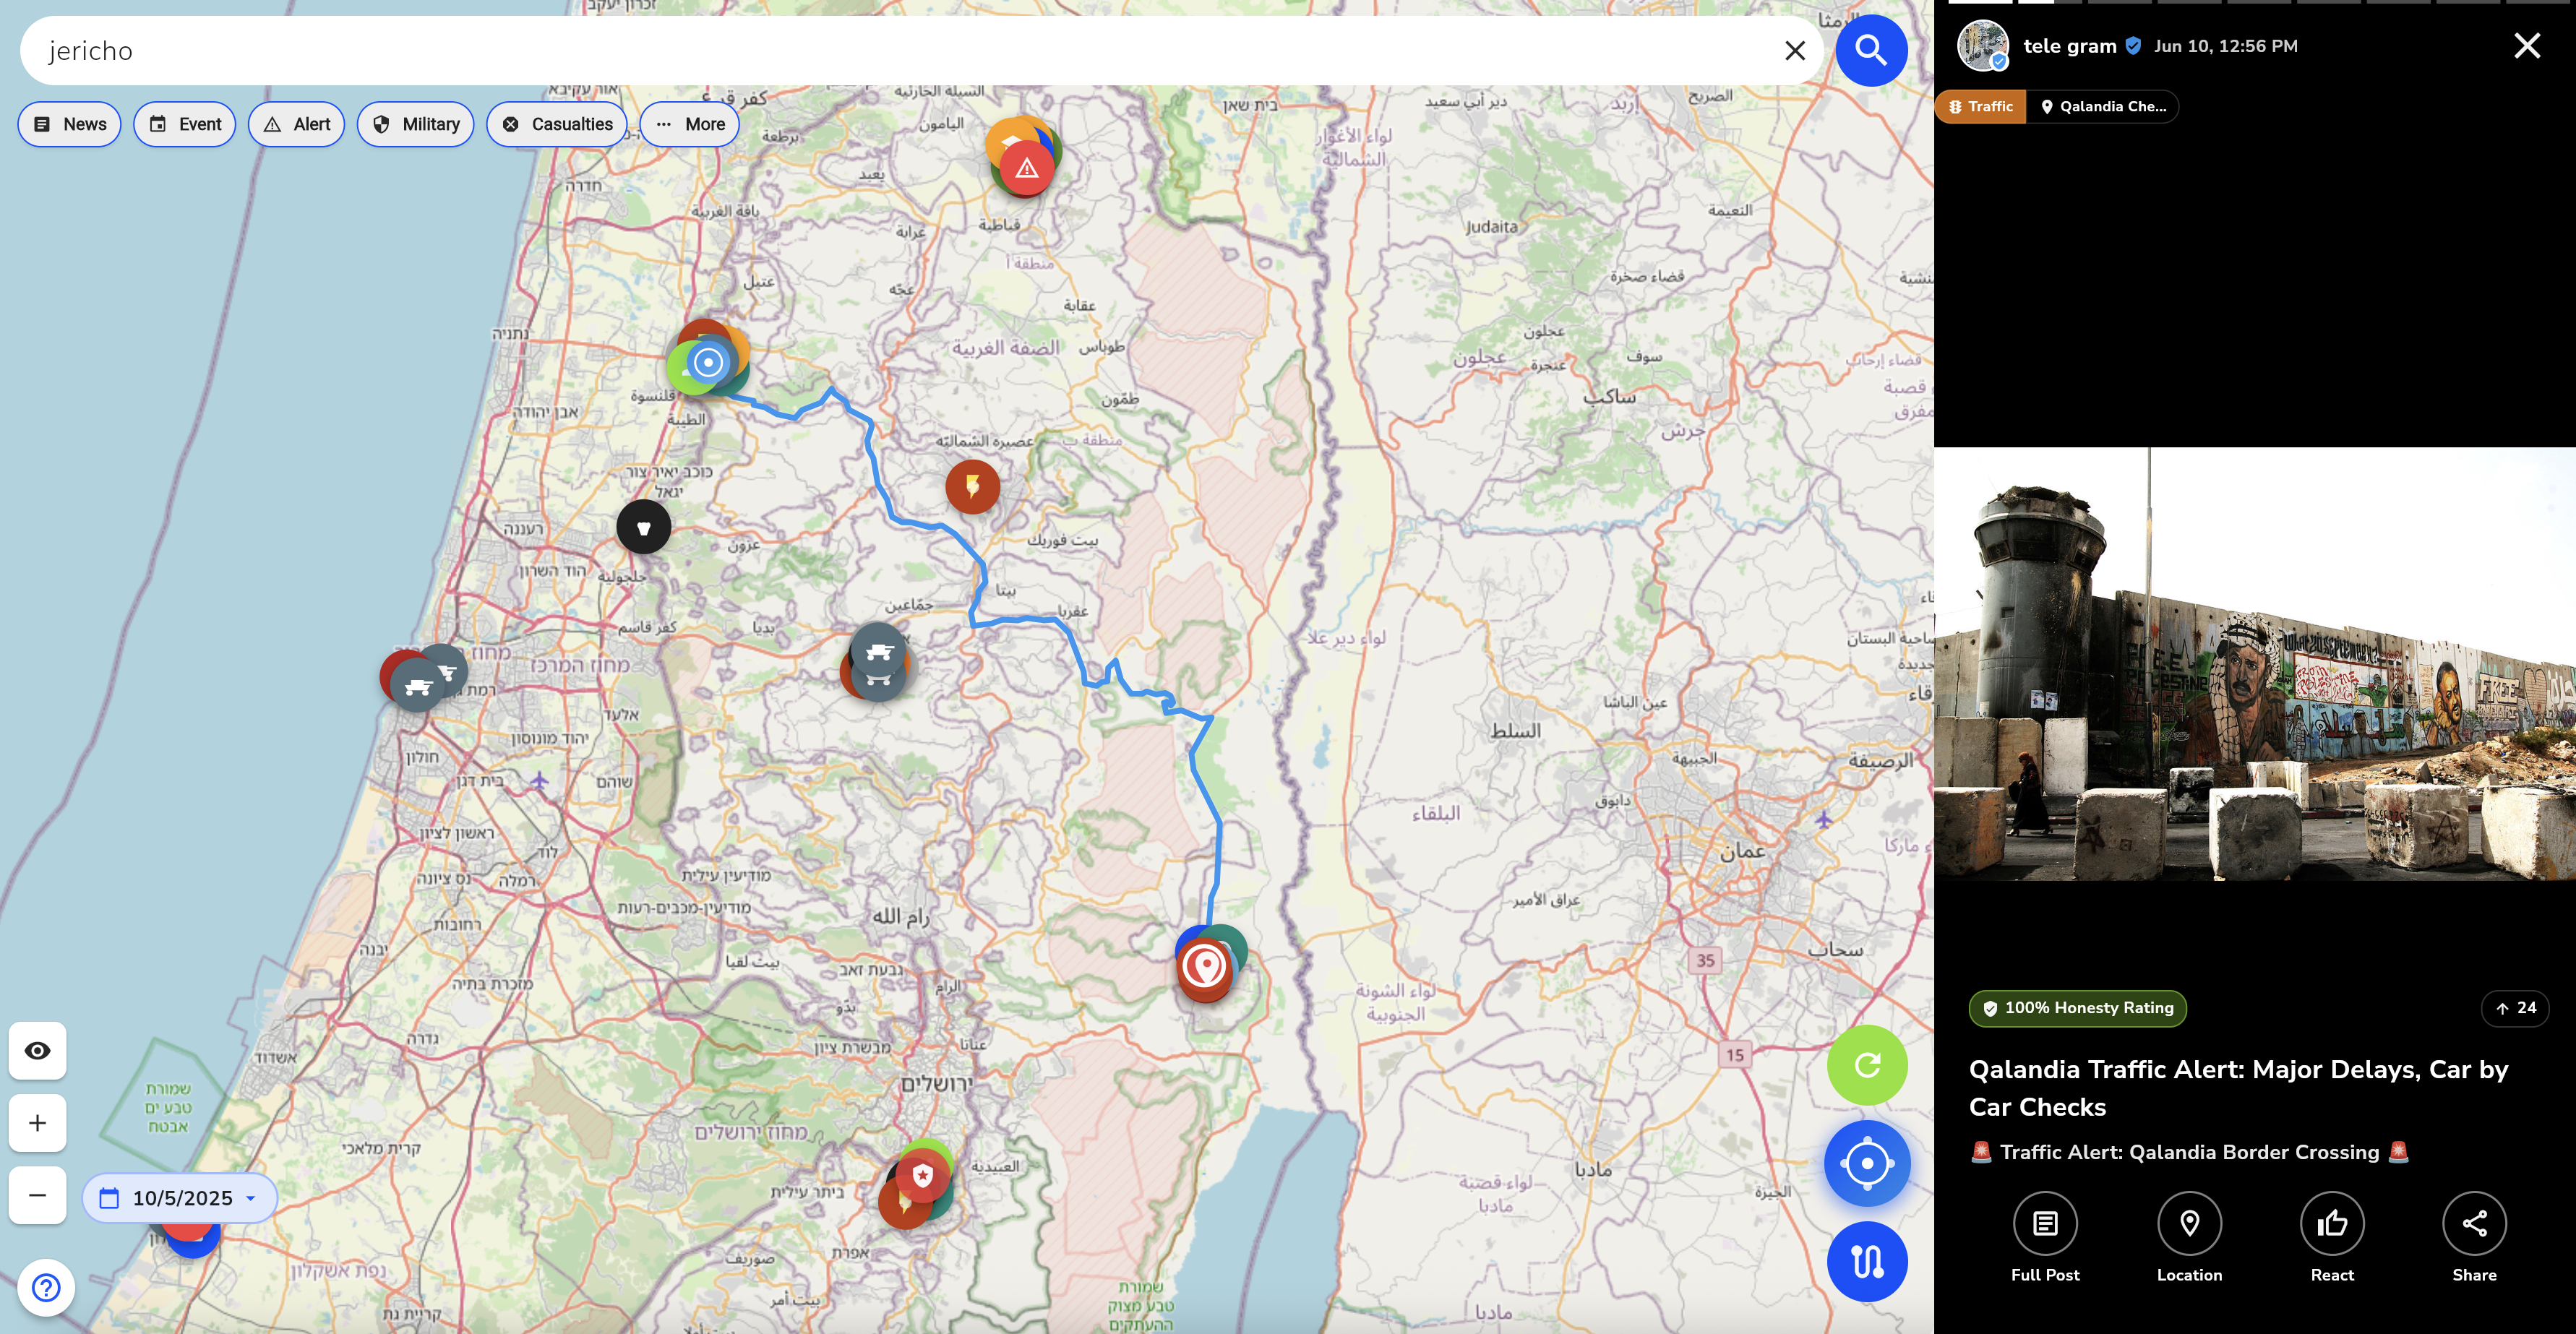
\includegraphics[width=1\textwidth]{figures/ui/Stories_web.png}
    \caption{Stories Integration on Web---Location-Based Story Discovery with Map Interface}\label{fig:web_stories}
\end{figure}

\clearpage

\paragraph{Interactive Map and Navigation Results}
The application delivers a comprehensive interactive mapping system providing users with location-based content discovery, navigation capabilities, and advanced geographic visualization. The map system successfully integrates real-time content, route planning, and intelligent search functionality.

\textbf{Mobile Interface (Android):}
The interactive mapping system provides comprehensive location-based functionality with content visualization, navigation tools, and advanced search capabilities for enhanced geographic interaction.

\begin{figure}[!htbp]
    \centering
    \subfigure[Interactive Map Interface]{
        \includegraphics[width=0.32\textwidth]{figures/ui/map_android.jpeg}
    }%
    \subfigure[Map Search Functionality]{
        \includegraphics[width=0.32\textwidth]{figures/ui/map_search.jpeg}
    }%
    \subfigure[Route Planning]{
        \includegraphics[width=0.32\textwidth]{figures/ui/map_route.jpeg}
    }
    \caption{Core Map Features---Interactive Interface, Search, and Navigation}\label{fig:android_map_core}
\end{figure}




\begin{figure}[!htbp]
    \centering
    \subfigure[Map Reels Discovery]{
        \includegraphics[width=0.45\textwidth]{figures/ui/map_reels_androidn.jpeg}
    }
    \hspace{0.05\textwidth}
    \subfigure[Map Legend and Categories]{
        \includegraphics[width=0.45\textwidth]{figures/ui/map_legend.jpeg}
    }
    \caption{Advanced Map Features---Content Discovery and Category Visualization}\label{fig:android_map_advanced}
\end{figure}

The interactive mapping system delivers comprehensive location-based functionality with advanced features for content discovery, navigation, and community interaction:

\textbf{Advanced Map Interface Features:}
\begin{itemize}
    \item \textbf{Intelligent Pin System:} Dynamic location pins with category-specific icons showing real-time content distribution across geographic areas with color-coded indicators for different content types (News, Events, Alerts, Military, Casualties)
    \item \textbf{Home Router Integration:} Automated location detection with home base functionality allowing users to set primary locations and receive proximity-based content recommendations with distance calculations
    \item \textbf{Interactive Route Planning:} Turn-by-turn navigation with optimized routing algorithms supporting multiple waypoints, traffic-aware pathfinding, and location-based content discovery along routes
    \item \textbf{Advanced Search Capabilities:} Geographic search functionality with address resolution, coordinate input, and landmark recognition for efficient location discovery
\end{itemize}
\clearpage

\textbf{Content Discovery and Interaction:}
\begin{itemize}
    \item \textbf{Comprehensive Category System:} Full content categorization including News, Events, Alerts, Politics, Sports, Health, Traffic, Weather, Crime, Community, Disaster, Environment, Education with distinct visual markers and filtering capabilities
    \item \textbf{Multi-Modal Content Access:} Flexible content viewing options allowing users to switch between full post details, media-only displays, summary cards, and location-focused views with customizable information density
    \item \textbf{Interactive Content Panels:} Slide-up content panels with rich media display, engagement metrics, sharing capabilities, and contextual actions without leaving the map interface
    \item \textbf{Geographic Content Threading:} Automatic grouping of related content by location proximity with timeline visualization and event correlation for comprehensive situation awareness
    \item \textbf{Community Engagement Mapping:} User-generated content integration with community verification, honesty ratings, and collaborative fact-checking displayed with geographic context and credibility indicators
\end{itemize}

\textbf{Advanced Visualization and Controls:}
\begin{itemize}
    \item \textbf{Dynamic Layer Management:} Multiple map layers supporting satellite imagery, street view integration, topographic overlays, and custom content layers with seamless switching and opacity controls
    \item \textbf{Temporal Content Filtering:} Time-based content discovery allowing users to view historical events, current activities, and scheduled future content with timeline scrubbing and temporal analysis
    \item \textbf{Proximity-Based Notifications:} Location-aware alert system providing context-sensitive notifications for nearby events, breaking news, and community activities with customizable radius settings
    \item \textbf{Advanced Map Legend:} Comprehensive symbol directory with interactive legend showing all content categories, special incident markers (casualties, explosions, military, fire), and user-customizable display preferences
    \item \textbf{Multi-Touch Interaction:} Gesture-based navigation with pinch-to-zoom, rotation support, multi-finger pan, and contextual tap actions for seamless map exploration and content interaction
\end{itemize}

\clearpage

\paragraph{Notifications Management Results}
The application delivers a comprehensive notifications system providing users with real-time updates and flexible management options.

\textbf{Mobile Interface (Android):}
The notifications system provides centralized notification management, in-app alerts, bulk actions, and swipe-to-action controls for efficient notification handling.

\begin{figure}[!htbp]
    \centering
    \subfigure[Main Notifications Dashboard]{
        \includegraphics[width=0.32\textwidth]{figures/ui/notfications_android.jpeg}
    }%
    \subfigure[Dedicated Notification List]{
        \includegraphics[width=0.32\textwidth]{figures/ui/notfication_list_android.jpeg}
    }%
    \subfigure[In-App Snackbar Notification]{
        \includegraphics[width=0.32\textwidth]{figures/ui/notification_snackbar_insidetheapp.jpeg}
    }
    \caption{Notifications Interface---Dashboard, List View, and In-App Alerts}\label{fig:android_notifications_core}
\end{figure}

The notification system demonstrates robust real-time capabilities with continuous event monitoring and intelligent delivery mechanisms. Notifications for ongoing events are marked as "still happening" to maintain relevance and user awareness. The system successfully delivers foreground notifications when users are actively using the application, providing immediate visual feedback through snackbar alerts and in-app notifications. Background notifications ensure users remain informed even when the application is not in active use, leveraging Firebase Cloud Messaging for reliable push delivery across device states and network conditions.

\clearpage

\begin{figure}[!htbp]
    \centering
    \subfigure[Management Options Sheet]{
        \includegraphics[width=0.32\textwidth]{figures/ui/notifications_options_bottom_sheet_markall_and_open_settings_option.jpeg}
    }%
    \subfigure[Swipe Actions: Delete/Mark]{
        \includegraphics[width=0.32\textwidth]{figures/ui/notifications_swipe_options_delete_markas.jpeg}
    }%
    \subfigure[Foreground Notification Reception]{
        \includegraphics[width=0.32\textwidth]{figures/ui/reciving_notificaition_android_foreground.jpeg}
    }
    \caption{Advanced Notifications Management---Bulk Actions, Swipe Controls, and Real-Time Reception}\label{fig:android_notifications_advanced}
\end{figure}

\textbf{Web Platform Achievement:}
The web notifications system provides enhanced desktop experience with larger screen real estate for comprehensive notification management, optimized for keyboard navigation and multi-panel interfaces.

\begin{figure}[!htbp]
    \centering
    \includegraphics[width=1\textwidth]{figures/ui/notifcations_page_web.png}
    \caption{Notifications Management on Web---Desktop Interface with Enhanced Functionality}\label{fig:web_notifications}
\end{figure}

\paragraph{Content Systems Results}
The application delivers two distinct content systems: external news aggregation from trusted web sources and user-generated community posts. These systems operate independently while providing comprehensive content discovery and interaction capabilities.

\textbf{Mobile Interface (Android):}
\begin{figure}[!htbp]
    \centering
    \subfigure[News From Around the Web]{
        \includegraphics[width=0.45\textwidth]{figures/ui/all_news_from_around_web_phone.jpeg}
    }
    \hspace{0.05\textwidth}
    \subfigure[External Article Integration]{
        \includegraphics[width=0.45\textwidth]{figures/ui/news_from_web_brief_details_phone.jpeg}
    }
    \caption{External News Aggregation and Article Integration on Android---Third-Party Content Discovery}\label{fig:android_news_map}
\end{figure}

\begin{figure}[!htbp]
    \centering
    \subfigure[User Post Detail View]{
        \includegraphics[width=0.45\textwidth]{figures/ui/Post_details_phone.jpeg}
    }
    \hspace{0.05\textwidth}
    \subfigure[User Posts Feed Interface]{
        \includegraphics[width=0.45\textwidth]{figures/ui/all_posts_page_with_filters.jpeg}
    }
    \caption{User-Generated Posts System on Android---Community Content and Interaction Features}\label{fig:android_post_details}
\end{figure}

\textbf{External News Aggregation System:}
The "News From Around the Web" feature aggregates content from external trusted sources (Fox News, BBC News, CNN, The Washington Post, Post Magazine) providing users with curated external articles. This system operates independently from user-generated content, offering seamless "Read Full Article" functionality that connects users directly to original news sources while maintaining app context.

\textbf{User-Generated Posts System:}
The user posts interface provides comprehensive community-driven content management with sophisticated filtering and interaction capabilities. Key features include dynamic date filtering (10/5/2025), intelligent sorting mechanisms (Popular, Latest, Most Upvoted, Verified Only), comprehensive category systems (All, News, Event), and rich content cards with location context (Neve Ze'ev, Beersheba, Palestine). 

User posts feature complete community interaction tools including upvote/downvote systems, community honesty ratings (91\%, 90\%), save/unsave functionality, sharing capabilities, comment threading, and location-based content organization. This system enables users to create, discover, and engage with community-generated content through location-verified posting and comprehensive engagement metrics.

\textbf{Social Networking and User Discovery:}
The application delivers comprehensive social networking capabilities with advanced user discovery, profile interactions, and community building features. The social system integrates seamlessly with location-based content discovery while providing robust following and interaction mechanisms.

\begin{figure}[!htbp]
    \centering
    \subfigure[User Profile Posts View]{
        \includegraphics[width=0.45\textwidth]{figures/ui/posts_from_somoeones_profile.jpeg}
    }
    \hspace{0.05\textwidth}
    \subfigure[Follow Features and User Discovery]{
        \includegraphics[width=0.45\textwidth]{figures/ui/other_ppl_profile_andfollowbutton_anddiscoverppl.jpeg}
    }
    \caption{Social Profile Features---User Content Discovery and Community Interaction}\label{fig:android_social_profiles}
\end{figure}

\begin{figure}[!htbp]
    \centering
    \subfigure[Search Posts and People]{
        \includegraphics[width=0.45\textwidth]{figures/ui/search_posts_and_ppl.jpeg}
    }
    \hspace{0.05\textwidth}
    \subfigure[Following List Management]{
        \includegraphics[width=0.45\textwidth]{figures/ui/following_list.jpeg}
    }
    \caption{Social Discovery Features---Search Functionality and Follow Management}\label{fig:android_social_discovery}
\end{figure}

The social networking implementation showcases sophisticated community-building features:

\textbf{Profile-Based Content Discovery:}
The user profile system provides comprehensive content access through dedicated profile pages showing individual user's posts, activities, and content contributions. Users can explore other members' content through clean, organized profile interfaces that maintain location context while showcasing user-generated content and community engagement metrics.

\textbf{Advanced Follow System:}
The follow functionality enables users to build personalized networks with clear follow/unfollow controls, follower discovery mechanisms, and suggested user recommendations. The system includes smart user discovery featuring "Discover People" functionality that suggests relevant users based on location proximity, shared interests, and community activity patterns.

\textbf{Comprehensive Search Capabilities:}
The unified search system allows users to discover both content and people through intelligent search algorithms. Users can search for posts based on content, location, and category while simultaneously discovering relevant community members, creating seamless content and social discovery experiences.

\textbf{Following Management Interface:}
The following list management provides organized access to user networks with comprehensive follower/following lists, user status indicators, and relationship management tools. The interface includes search functionality within following lists, user activity status displays, and efficient relationship management for growing community networks.

\textbf{Community Engagement Features:}
The social system integrates engagement metrics throughout user interactions, including follow counts, mutual connections, activity status indicators, and community reputation scores. Users can discover trending community members, explore popular content creators, and build meaningful connections based on shared location interests and content preferences.

\paragraph{Feature Implementation Summary}
The application delivers comprehensive functionality across all core areas:

\begin{itemize}
    \item \textbf{Location Verification:} GPS-based content authentication with range-based posting restrictions enhancing community trust and information reliability
    \item \textbf{Real-time Communication:} Instant messaging with conversation threading, smart assistant integration, and reliable message synchronization
    \item \textbf{Content Management:} Intelligent post categorization, effective filtering, automated threading, and location-aware content recommendations with community honesty scoring
    \item \textbf{Smart Assistant:} Location-aware recommendations, personalized content discovery, real-time news integration, and contextual assistance for platform navigation
    \item \textbf{Cross-Platform Consistency:} Responsive design adapting to various screen sizes with accessibility features including proper contrast ratios and screen reader support
\end{itemize}
\clearpage
\section{Results Summary}\label{sec:results_summary}

The results presented in this chapter demonstrate the successful implementation of LiveSpot as a comprehensive, location-based social networking platform that effectively addresses the challenges of information verification and community-driven content management. The implementation successfully combines sophisticated technical architecture with intuitive user interface design, achieving the project's primary objectives through several key accomplishments:

\textbf{Cross-Platform Achievement:}
LiveSpot successfully delivers consistent user experience across Android, iOS, and web platforms with comprehensive feature parity. The achieved cross-platform implementation ensures users receive identical functionality regardless of their chosen platform, demonstrating successful technology integration.

\textbf{User Interface Excellence:}
The delivered interface achieves exceptional design consistency with responsive layouts adapting seamlessly across device sizes. The comprehensive theming system provides both light and dark mode experiences while maintaining accessibility compliance and user choice.

\textbf{Smart Assistant Innovation:}
The Smart Assistant provides intelligent, location-aware recommendations enhancing user engagement through personalized content discovery. The system successfully combines location intelligence with user preferences to deliver contextual assistance and community engagement features.

\textbf{News Aggregation and Content Discovery Innovation:}
The implementation successfully delivers comprehensive news aggregation from multiple trusted sources (Fox News, BBC News, CNN, The Washington Post, Post Magazine) through the "From Around the Web" feature. The system provides intelligent content categorization, real-time updates, and seamless external article access while maintaining app context. The interactive map legend demonstrates sophisticated content visualization with comprehensive category coverage and special incident indicators for critical events.

\textbf{Advanced Post Interaction System:}
The post detail interface achieves comprehensive content engagement with working upvote/downvote systems, community-driven honesty ratings, multi-platform sharing capabilities, and save/unsave functionality. The implementation includes embedded geographic context, comment threading, and real-time event status tracking, providing users with complete content interaction capabilities within a location-aware framework.

\textbf{Smart Assistant Innovation:}
The Smart Assistant integration represents a significant innovation in location-based social networking, providing users with intelligent recommendations based on geographic context, personal interests, and community activity. The system successfully combines algorithmic processing with location intelligence to deliver personalized content discovery and community engagement features that enhance the overall user experience.

The comprehensive implementation results validate the effectiveness of the design decisions, demonstrating that LiveSpot successfully delivers sophisticated functionality through user-friendly interfaces. The platform provides a complete solution for location-based social networking and information verification, meeting all primary objectives while establishing a foundation for community-driven content verification and location-based social interaction.
